\section{Experiments}
\label{sec:experiments}

In this section, we show that DDIMs outperform DDPMs in terms of image generation when fewer iterations are considered, giving speed ups of $10\times$ to $100\times$ over the original DDPM generation process. %
Moreover, unlike DDPMs, once the initial latent variables $\vx_T$ are fixed, DDIMs retain high-level image features regardless of the generation trajectory, so they are able to perform interpolation directly from the latent space. DDIMs can also be used to encode samples that reconstruct them from the latent code, which DDPMs cannot do due to the stochastic sampling process.

For each dataset, we use the \textbf{same trained model} with $T = 1000$ and the objective being $L_\gamma$ from \eqref{eq:l-gamma} with $\gamma = \vone$; as we argued in Section~\ref{sec:variational}, no changes are needed with regards to the training procedure.
The only changes that we make is \textbf{how we produce samples from the model}; we achieve this by controlling $\tau$ (which controls how fast the samples are obtained) and $\sigma$ (which interpolates between the deterministic DDIM and the stochastic DDPM).

We consider different sub-sequences $\tau$ of $[1, \ldots, T]$ and different variance hyperparameters $\sigma$ indexed by elements of $\tau$. To simplify comparisons, we consider $\sigma$ with the form:
\begin{align}
    \sigma_{\tau_{i}}(\eta) = \eta \sqrt{(1 - \alpha_{\tau_{i-1}})/(1 - \alpha_{\tau_{i}})}\sqrt{1 - {\alpha_{\tau_i}}/{\alpha_{\tau_{i-1}}}}, %
\end{align}
where $\eta \in \R_{\geq 0}$ is a hyperparameter that we can directly control. This includes an original DDPM generative process when $\eta = 1$ and DDIM when $\eta = 0$. We also consider DDPM where the random noise has a larger standard deviation than $\sigma(1)$, which we denote as $\hat{\sigma}$:
$
    \hat{\sigma}_{\tau_{i}} = \sqrt{1 - {\alpha_{\tau_i}}/{\alpha_{\tau_{i-1}}}}%
$
. This is used by \href{https://github.com/hojonathanho/diffusion/blob/master/scripts/run_cifar.py#L136}{\underline{the implementation}} in \cite{ho2020denoising} \textbf{only to obtain the CIFAR10 samples}, but not samples of the other datasets. We include more details in Appendix~\ref{app:exp}. %

\subsection{Sample quality and efficiency}
In Table~\ref{tab:cifar10-fid}, we report the quality of the generated samples with models trained on CIFAR10 and CelebA, as measured by Frechet  Inception Distance (FID~\citep{heusel2017gans}), where we vary the number of timesteps used to generate a sample ($\dim(\tau)$) and the stochasticity of the process ($\eta$).
As expected, the sample quality becomes higher as we increase $\dim(\tau)$, presenting a trade-off between sample quality and computational costs.
We observe that DDIM ($\eta = 0$) achieves the best sample quality when $\dim(\tau)$ is small, and DDPM ($\eta = 1$ and $\hat{\sigma}$) typically has worse sample quality compared to its less stochastic counterparts with the same $\dim(\tau)$, except for the case for $\dim(\tau) = 1000$ and $\hat{\sigma}$ reported by \citet{ho2020denoising} where DDIM is marginally worse. However, the sample quality of $\hat{\sigma}$ becomes much worse for smaller $\dim(\tau)$, which suggests that it is ill-suited for shorter trajectories. DDIM, on the other hand, achieves high sample quality much more consistently. 

In \Figref{fig:cifar10-tvh}, we show CIFAR10 and CelebA samples with the same number of sampling steps and varying $\sigma$. For the DDPM, the sample quality deteriorates rapidly when the sampling trajectory has 10 steps. For the case of $\hat{\sigma}$, the generated images seem to have more noisy perturbations under short trajectories; this explains why the FID scores are much worse than other methods, as FID is very sensitive to such perturbations (as discussed in \citet{Jolicoeur-Martineau2020adversarial}). 

In \Figref{fig:time}, we show that the amount of time needed to produce a sample scales linearly with the length of the sample trajectory. %
This suggests that DDIM is useful for producing samples more efficiently, as samples can be generated in much fewer steps. Notably, DDIM is able to produce samples with quality comparable to 1000 step models within $20$ to $100$ steps, which is a $10\times$ to $50\times$ speed up compared to the original DDPM. Even though DDPM could also achieve reasonable sample quality with $100\times$ steps, DDIM requires much fewer steps to achieve this; on CelebA, the FID score of the 100 step DDPM is similar to that of the 20 step DDIM. 

\newcolumntype{G}{>{\centering}b{0.065\textwidth}}
\newcolumntype{C}{>{\centering\arraybackslash}b{0.065\textwidth}}
\definecolor{LightCyan}{rgb}{0.88,1,1}
\definecolor{LightOrange}{rgb}{1,0.85,0.70}
\definecolor{DarkCyan}{rgb}{0,0.8,0.8}
\definecolor{DarkOrange}{rgb}{1,0.50,0.0}
\begin{table}
    \centering
    \caption{CIFAR10 and CelebA image generation measured in FID. $\eta = 1.0$ and $\hat{\sigma}$ are cases of {\color{DarkOrange}DDPM} (although \citet{ho2020denoising} only considered $T=1000$ steps, and $S < T$ can be seen as simulating DDPMs trained with $S$ steps), and $\eta = 0.0$ indicates {\color{DarkCyan}DDIM}. %
    }
    \resizebox{\textwidth}{!}{
    \begin{tabular}{lc|GGGGG|GGGGC}
    \toprule
    &  & \multicolumn{5}{c|}{CIFAR10 ($32 \times 32$)} & \multicolumn{5}{c}{CelebA ($64 \times 64$)} \\
    \multicolumn{2}{c|}{$S$} & 10 & 20 & 50 & 100 & 1000 & 10 & 20 & 50 & 100 & 1000 \\\midrule
    \rowcolor{LightCyan}
    \multirow{4}{*}{$\eta$} & $0.0$ & \textbf{13.36} & \textbf{6.84} & \textbf{4.67} & \textbf{4.16} & 4.04 & \textbf{17.33} & \textbf{13.73} & \textbf{9.17} & \textbf{6.53} & 3.51 \\
    & 0.2 & 14.04 & 7.11 & 4.77 & 4.25 & 4.09 & 17.66 & 14.11 & 9.51 & 6.79 & 3.64 \\
    & 0.5 & 16.66 & 8.35 & 5.25 & 4.46 & 4.29 & 19.86 & 16.06 & 11.01 & 8.09 & 4.28 \\
    \rowcolor{LightOrange}
    & 1.0 & 41.07 & 18.36 & 8.01 & 5.78 & 4.73  & 33.12 & 26.03 & 18.48 & 13.93 & 5.98 \\\midrule
    \rowcolor{LightOrange}
    \multicolumn{2}{c|}{$\hat{\sigma}$} & 367.43 & 133.37 & 32.72 & 9.99 & \textbf{3.17} & 299.71 & 183.83 & 71.71 & 45.20 & \textbf{3.26} \\
        \bottomrule
    \end{tabular}
    }
    \label{tab:cifar10-fid}
\end{table}

\begin{figure}
    \centering
    \begin{subfigure}{0.23\textwidth}
    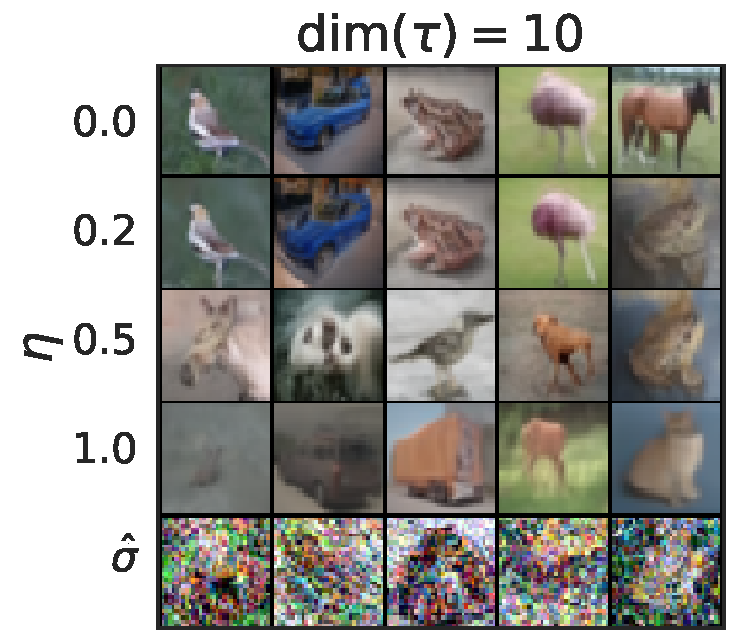
\includegraphics[width=\textwidth]{figures/cifar10-dim10.pdf}
    \end{subfigure}
    ~
    \begin{subfigure}{0.23\textwidth}
    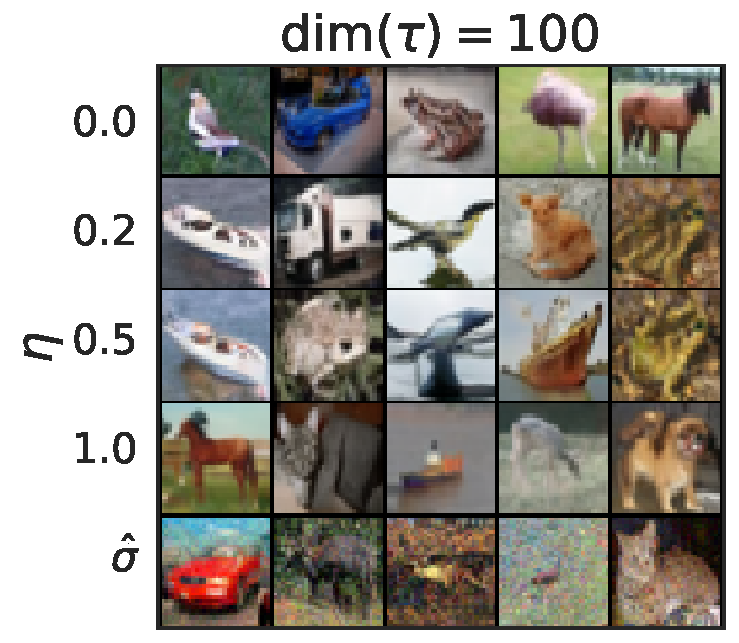
\includegraphics[width=\textwidth]{figures/cifar10-dim100.pdf}
    \end{subfigure}
    ~
        \begin{subfigure}{0.23\textwidth}
    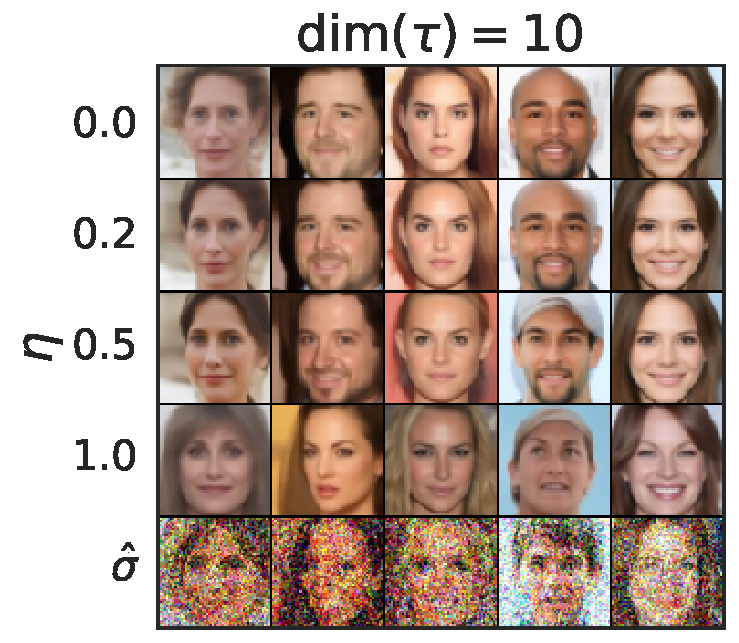
\includegraphics[width=\textwidth]{figures/celeba-dim10.pdf}
    \end{subfigure}
    ~
    \begin{subfigure}{0.23\textwidth}
    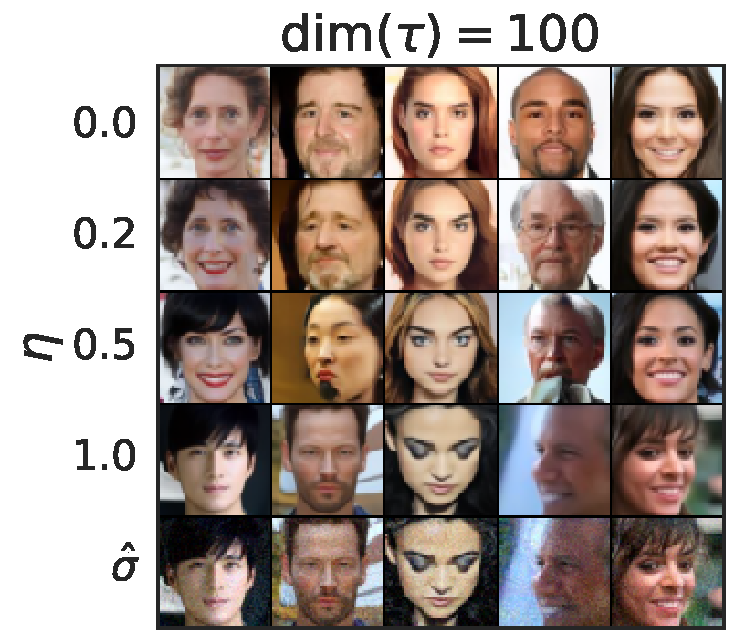
\includegraphics[width=\textwidth]{figures/celeba-dim100.pdf}
    \end{subfigure}
    \caption{CIFAR10 and CelebA samples with $\dim(\tau) = 10$ and $\dim(\tau) = 100$.}
    \label{fig:cifar10-tvh}
\end{figure}

\begin{figure}
    \centering
    \begin{subfigure}{0.4\textwidth}
    \centering
        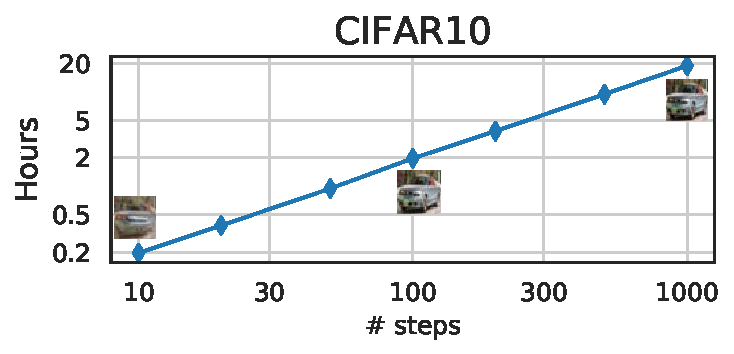
\includegraphics[width=\textwidth]{figures/cifar10-tvh.pdf}
    \end{subfigure}
    ~
     \begin{subfigure}{0.4\textwidth}
     \centering
        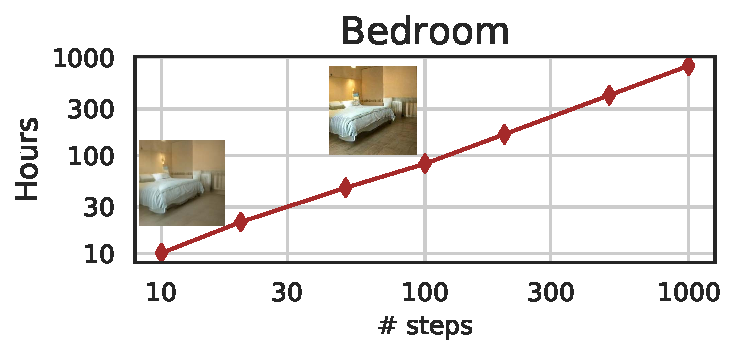
\includegraphics[width=\textwidth]{figures/bedroom-tvh.pdf}
    \end{subfigure}
    \caption{Hours to sample 50k images with one Nvidia 2080 Ti GPU and samples at different steps.}
    \label{fig:time}
\end{figure}

\subsection{Sample consistency in DDIMs} 
For DDIM, the generative process is deterministic, and $\vx_0$ would depend only on the initial state $\vx_T$. In \Figref{fig:consistency}, we observe the generated images under different generative trajectories (i.e. different $\tau$) while starting with the same initial $\vx_T$. Interestingly, for the generated images with the same initial $\vx_T$, most high-level features are similar, regardless of the generative trajectory. In many cases, samples generated with only 20 steps are already very similar to ones generated with 1000 steps in terms of high-level features, with only minor differences in details. 
Therefore, it would appear that $\vx_T$ alone would be an informative latent encoding of the image; and minor details that affects sample quality are encoded in the parameters, as longer sample trajectories gives better quality samples but do not significantly affect the high-level features.
We show more samples in Appendix~\ref{app:samples}. %

\begin{figure}
\begin{subfigure}{\textwidth}
    \centering
    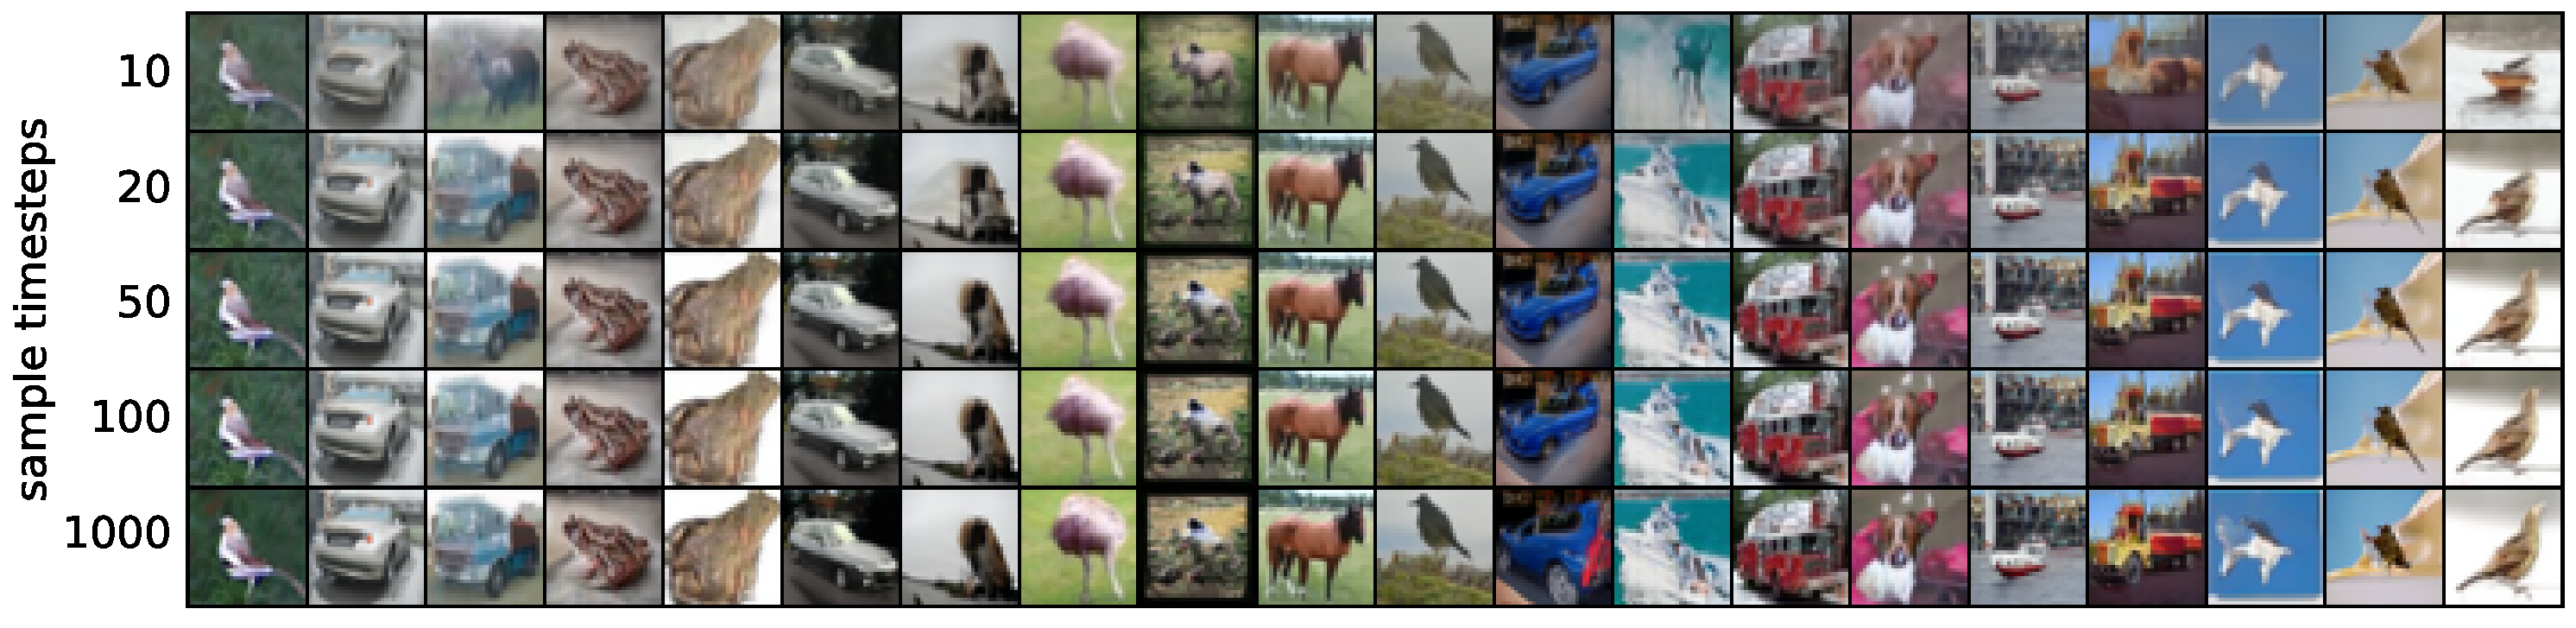
\includegraphics[width=0.95\textwidth]{figures/cifar10-consistency.pdf}
\end{subfigure}

\begin{subfigure}{\textwidth}
    \centering
    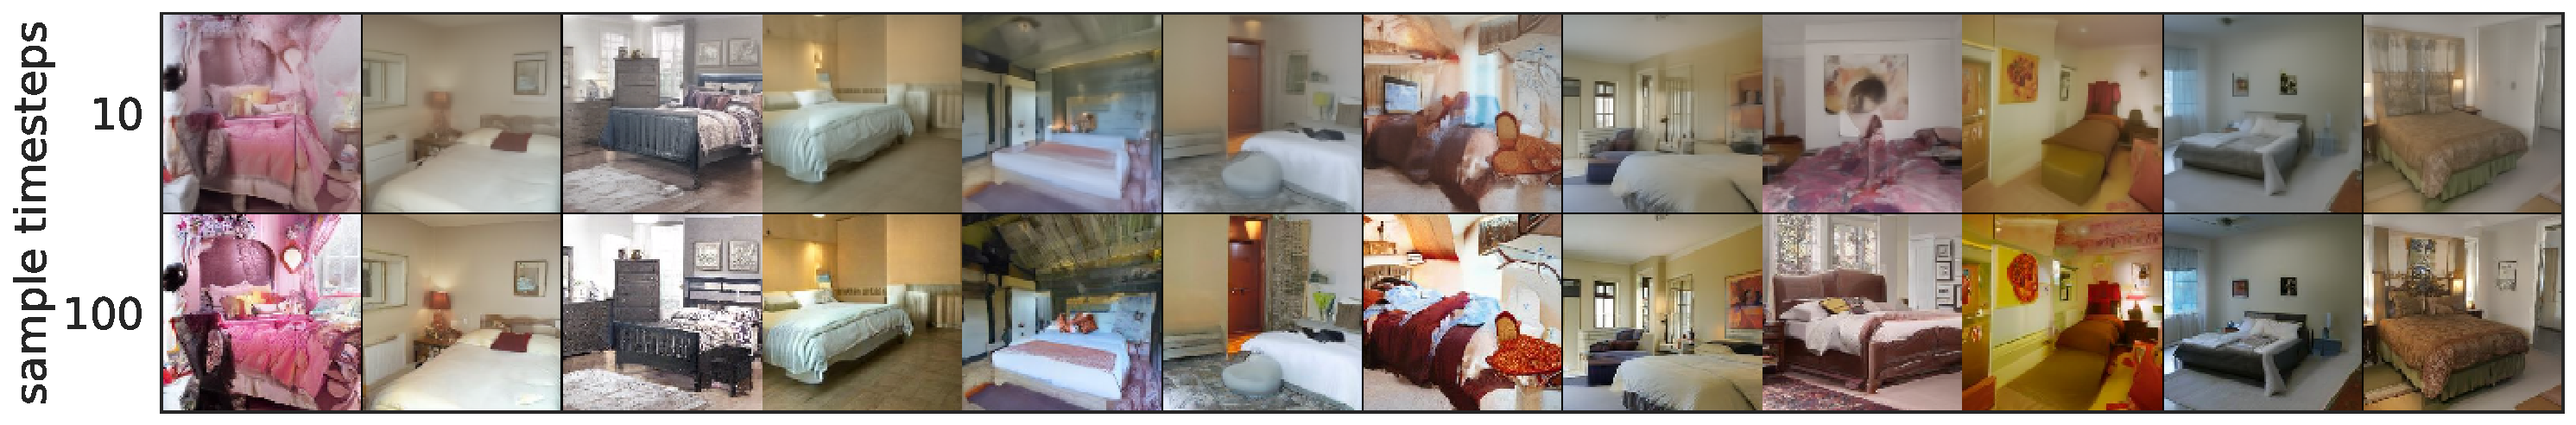
\includegraphics[width=0.99\textwidth]{figures/bedroom-consistency.pdf}
\end{subfigure}

\begin{subfigure}{\textwidth}
    \centering
    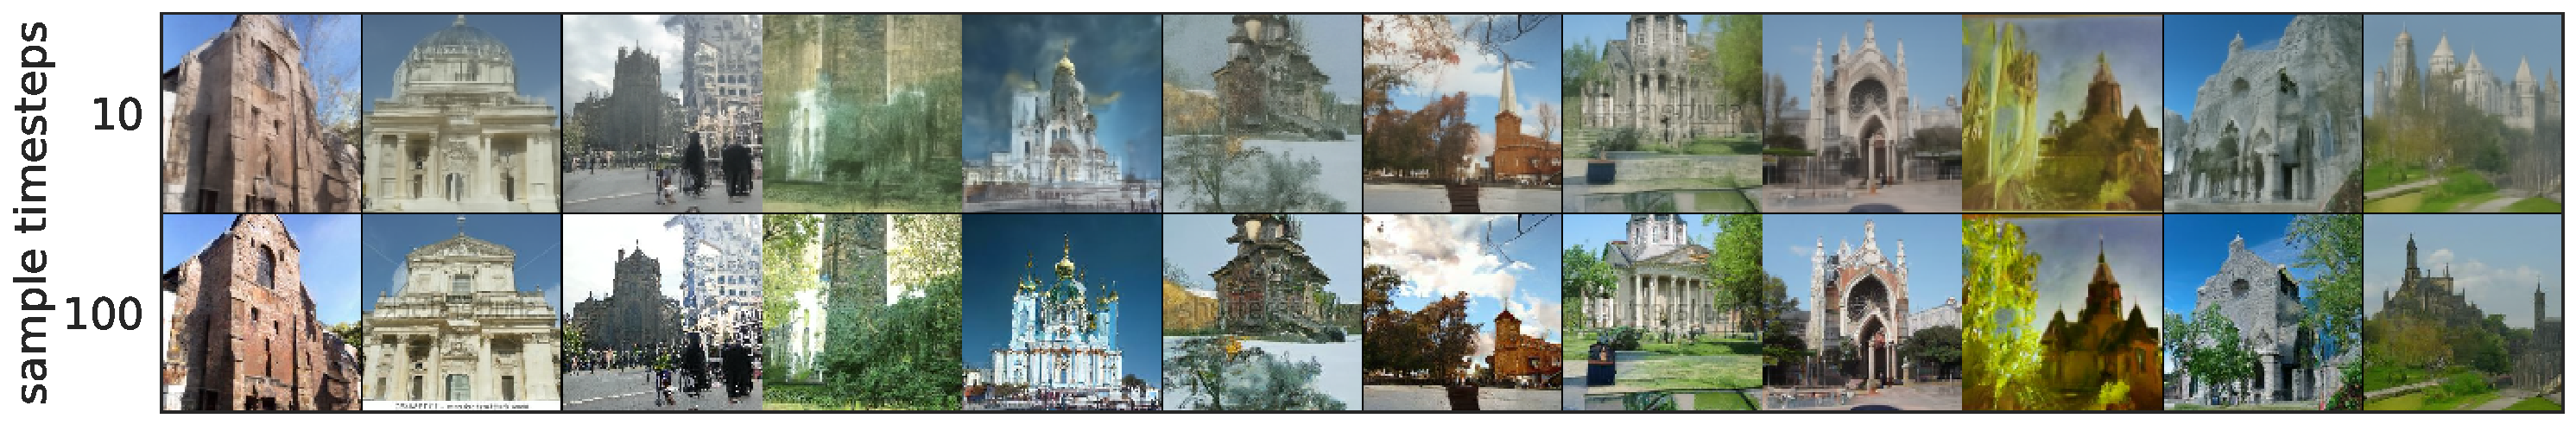
\includegraphics[width=0.99\textwidth]{figures/church-consistency.pdf}
\end{subfigure}
\caption{Samples from DDIM with the same random $\vx_T$ and different number of steps.}
\label{fig:consistency}
\end{figure}

\subsection{Interpolation in deterministic generative processes} 
\begin{figure}[h]
\begin{subfigure}{\textwidth}
    \centering
    
\includegraphics[width=\textwidth]{figures/celeba-interp-line.png}
\end{subfigure}
~
\begin{subfigure}{\textwidth}
    \centering
    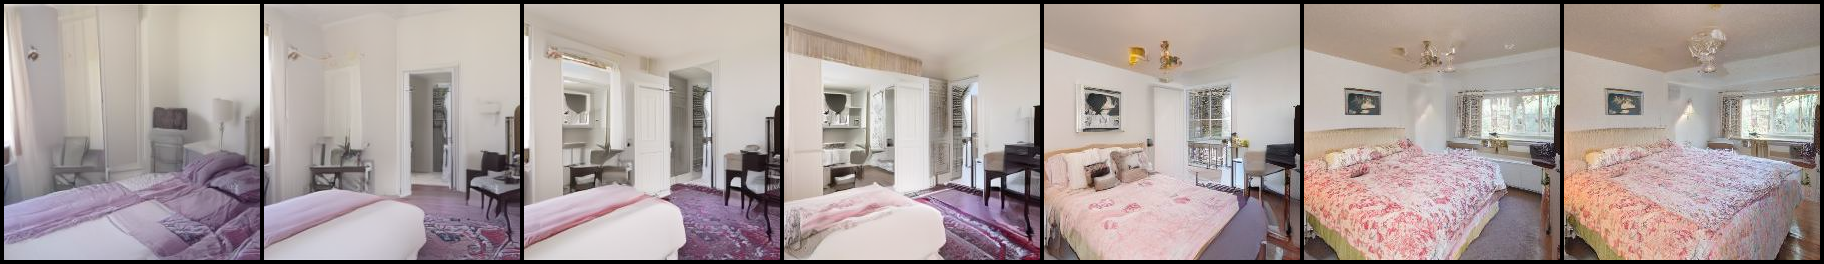
\includegraphics[width=\textwidth]{figures/bedroom-interp-line.png}
\end{subfigure}
~
\begin{subfigure}{\textwidth}
    \centering
    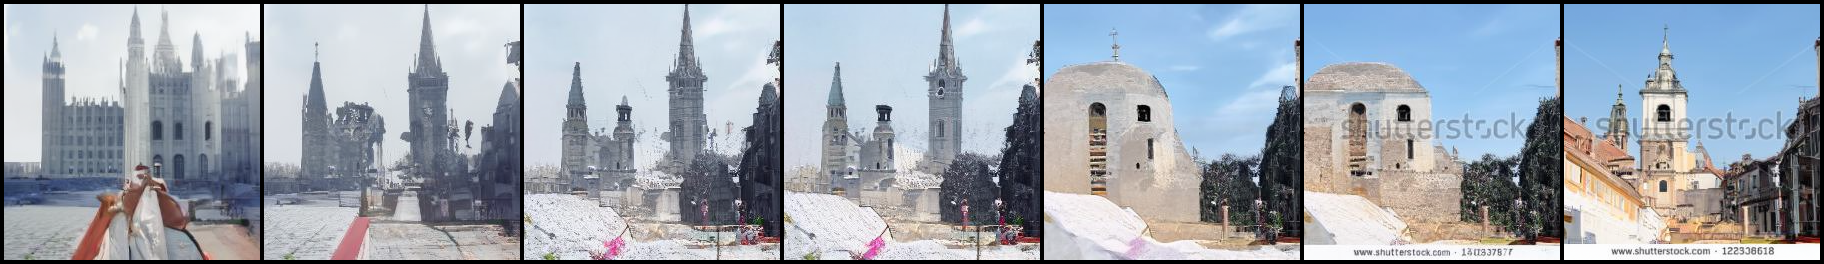
\includegraphics[width=\textwidth]{figures/church-interp-line.png}
\end{subfigure}
\caption{Interpolation of samples from DDIM with $\dim(\tau) = 50$.}
\label{fig:interp-line}
\end{figure}
Since the high level features of the DDIM sample is encoded by $\vx_T$, we are interested to see whether it would exhibit the semantic interpolation effect similar to that observed in other implicit probabilistic models, such as GANs~\citep{goodfellow2014generative}. This is different from the interpolation procedure in~\citet{ho2020denoising}, since in DDPM the same $\vx_T$ would lead to highly diverse $\vx_0$ due to the stochastic generative process\footnote{Although it might be possible if one interpolates all $T$ noises, like what is done in \citet{song2020improved}.}. In \Figref{fig:interp-line}, we show that simple interpolations in $\vx_T$ can lead to semantically meaningful interpolations between two samples. We include more details and samples in Appendix~\ref{app:interpolation}. This allows DDIM to control the generated images on a high level directly through the latent variables, which DDPMs cannot.

\subsection{Reconstruction from Latent Space}
As DDIM is the Euler integration for a particular ODE, it would be interesting to see whether it can encode from $\vx_0$ to $\vx_T$ (reverse of \eqref{eq:ddim-ode}) and reconstruct $\vx_0$ from the resulting $\vx_T$ (forward of \eqref{eq:ddim-ode})\footnote{Since $\vx_T$ and $\vx_0$ have the same dimensions, their compression qualities are not our immediate concern.}. We consider encoding and decoding on the CIFAR-10 test set with the CIFAR-10 model with $S$ steps for both encoding and decoding; we report the per-dimension mean squared error (scaled to $[0, 1]$) in Table~\ref{tab:cifar10-recon}. Our results show that DDIMs have lower reconstruction error for larger $S$ values and have properties similar to Neural ODEs and normalizing flows.
The same cannot be said for DDPMs due to their stochastic nature.
\begin{table}
    \centering
    \caption{Reconstruction error with DDIM on CIFAR-10 test set, rounded to $10^{-4}$.}
    \begin{tabular}{l|ccccccc}
    \toprule
    $S$ & 10 & 20 & 50 & 100 & 200 & 500 & 1000 \\
    \midrule
    Error & 0.014 & 0.0065 & 0.0023 & 0.0009 & 0.0004 & 0.0001 & $0.0001$ \\
    \bottomrule
    \end{tabular}
    \label{tab:cifar10-recon}
\end{table}